\documentclass[a4paper,12pt]{article}
% Deixar paginas Black 
%\usepackage{xcolor}
%\\pagecolor{black}
%\\color{white}
\usepackage[
  paperwidth=25.0cm,
  paperheight=400.0cm,
  left=1cm,
  right=1cm,
  top=0cm,
  bottom=0cm
]{geometry}
\usepackage{graphicx}  % No preâmbulo
\emergencystretch=3em
\hbadness=10000  % Ignora completamente underfull boxes
\tolerance=9999
% Pacotes básicos
%\usepackage[utf8]{inputenc}
\usepackage[T1]{fontenc}
\usepackage[brazil]{babel}
\usepackage{amsmath, amssymb}
\usepackage{hyperref}
\usepackage{xcolor}   % Necessário para cores

\title{\centering Algebra Linear com aplicações - pag.122}

\author{}
\date{}

\begin{document}
\maketitle{}

%{\centering 
\includegraphics[width=5cm]{ebook.jpg} \par}






\section*{algebra linear do pricipio ao verbo}
\section*{Historia...}
\section*{Frase marcante}
Conhecer algo nao é so saber como fuciona e sim entender todas as razoes de sua existencia, 
\section*{comessa aqui}






\section*{}
\begin{center}
\Huge \textbf{Flash-Card Session}
\end{center}
\vspace{1em} % Espaço vertical
\noindent
Nesta seção, denominada \textbf{Flash-Card Session}, serão armazenados e organizados todos os flash cards criados ao longo do estudo do livro. Cada flash card contém perguntas e respostas que ajudam a revisar e fixar os conceitos importantes abordados no material. 
O objetivo desta seção é fornecer uma forma prática de \textit{recall} ativo, permitindo que o leitor revise rapidamente os pontos principais do livro, reforçando o aprendizado de forma eficiente e contínua.
Recomendo este aplicativo para flash cards \textcolor{blue}{\textbf{\href{https://apps.ankiweb.net/}{https://apps.ankiweb.net/}}} 

\begin{center}
\colorbox{blue!30}{\Large\textbf{CAPÍTULO 1 - FUNCOES E MODELOS}}
\end{center}

\section*{Flash-Card 1 - Calculo Vol1 9Ed}
Qual é o objeto fundamental do cálculo\dotfill funções\\  
Quando uma função surge\dotfill quando uma quantidade depende de outra\\ 
Defina a notação de uma função\dotfill f(x)\\
Três coisas para formar uma função\dotfill conjunto A, conjunto B e uma regra de associação\\ 
Uma função associa a um único valor do contradomínio \dotfill verdade\\ 
Defina domínio\dotfill conjunto de valores que você pode colocar na função\\
Defina contradomínio\dotfill conjunto de valores que a função pode ter como saída\\
Defina imagem\dotfill conjunto de valores que a função realmente produz\\
Uma função deve associar a entrada a quantas saídas\dotfill uma única saída\\
O que é uma função \dotfill $\begin{aligned}{\centering 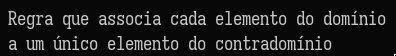
\includegraphics[width=7cm]{./res/image1.png}}\end{aligned}$\\ 
Faça o diagrama de máquina para uma função\dotfill$\begin{aligned}{\centering 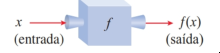
\includegraphics[width=7cm]{./res/image2.png}}\end{aligned}$\\
Defina: $\begin{aligned}{\centering 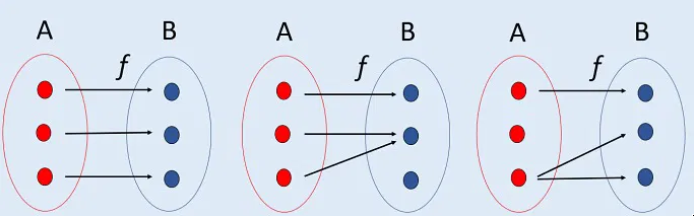
\includegraphics[width=7cm]{./res/image3.png}}\end{aligned}$\dotfill$\begin{aligned}{\centering 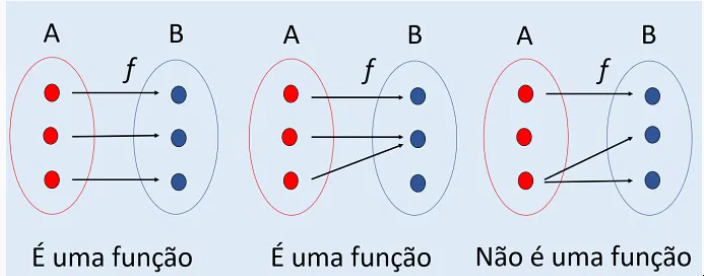
\includegraphics[width=7cm]{./res/image4.png}}\end{aligned}$\\ 
Defina: $\begin{aligned}{\centering 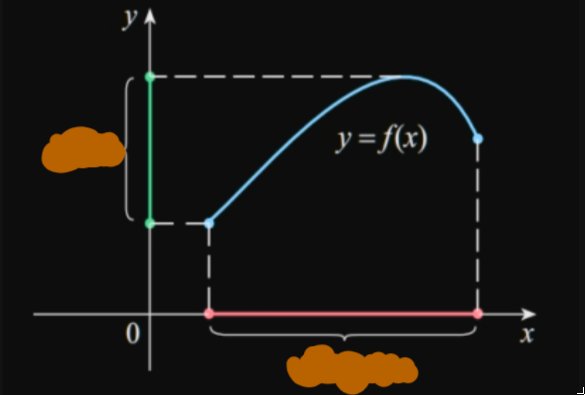
\includegraphics[width=7cm]{./res/image6.png}}\end{aligned}$\dotfill$\begin{aligned}{\centering 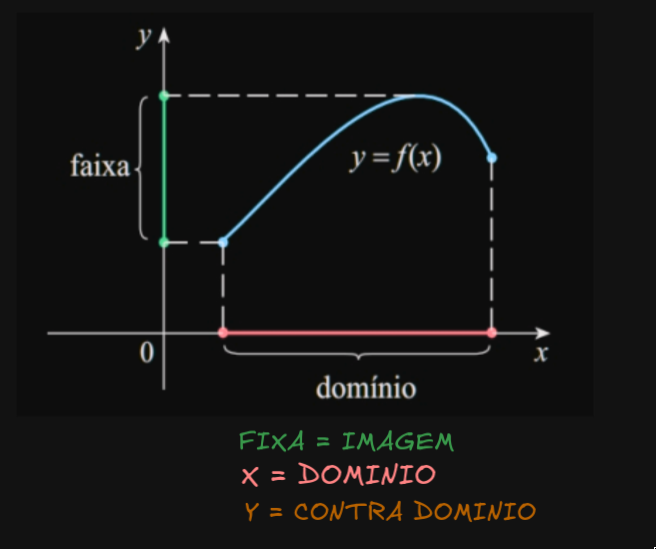
\includegraphics[width=7cm]{./res/image5.png}}\end{aligned}$\\

\section*{Flash-Card 2 - Calculo Vol1 9Ed}
Três tipos de funções\dotfill sobrejetora, injetora, bijetora\\
O que representa o quociente de diferença\dotfill taxa de variação média de uma função\\ 
Função sobrejetora\dotfill imagem = contradomínio\\
Função injetora\dotfill cada elemento da entrada tem uma imagem única\\
Função bijetora\dotfill injetora e sobrejetora\\
Quais valores o $h$ no quociente de diferença pode assumir\dotfill $h \neq 0$\\
Quociente de diferença fórmula\dotfill \fbox{$\frac{f(x+h) - f(x)}{h}$}\\ 

\section*{Flash-Card 3 - Calculo Vol1 9Ed}
Como se lê $\boxed{f: A \to B}$\dotfill f de A em B\\ 
função dentro de outra é chamada de\dotfill função composta\\ 
Qual o nome dessa fórmula \fbox{$\frac{f(x+h) - f(x)}{h}$}\dotfill quociente de diferença\\ 
função par\dotfill números opostos do domínio têm imagens iguais\\ 
função ímpar\dotfill números opostos do domínio têm imagens opostas\\ 
função ímpar: seu gráfico é\dotfill simétrico em relação à origem\\ 
função par: seu gráfico é\dotfill simétrico em relação ao eixo y\\ 
Defina função par ou ímpar $\begin{aligned}{\centering 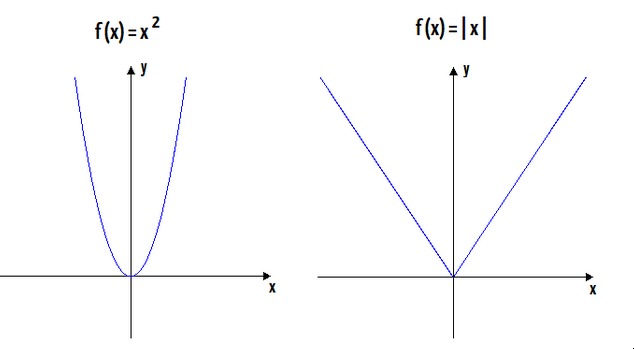
\includegraphics[width=4cm]{./res/image7.png}}\end{aligned}$\dotfill par\\ 
Defina função par ou ímpar $\begin{aligned}{\centering 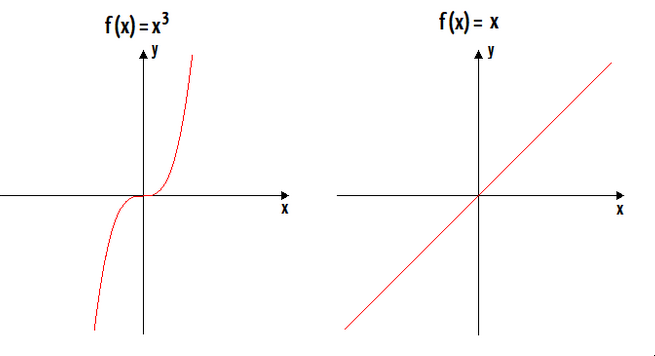
\includegraphics[width=4cm]{./res/image8.png}}\end{aligned}$\dotfill ímpar\\ 
Fórmula da função par e ímpar\dotfill$\boxed{\begin{aligned}\text{Função par:} \quad & f(-x) = f(x) \\\\\text{Função ímpar:} \quad & f(-x) = -f(x)\end{aligned}}$\\ 

\section*{Flash-Card 4 - Calculo Vol1 9Ed}
Condicao para um funcao ter inversa\dotfill precisa ser bijetora\\ 
como se ler isso $f \circ g$\dotfill f composta de g\\ 
notacao $f \circ g$\dotfill$f \circ g(x) = g(f(x))$\\ 
Notacao de funcao inversa\dotfill$\boxed{f(x) = y \;\;\Longleftrightarrow\;\; f^{-1}(y) = x}$\\
faca o diagrama de funcao composta:\dotfill$\begin{aligned}{\centering 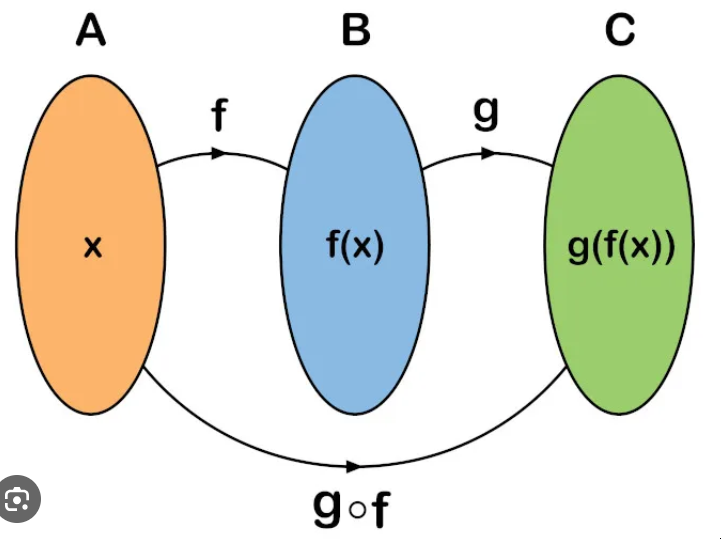
\includegraphics[width=5cm]{./res/image9.png}}\end{aligned}$\\

\section*{Flash-Card 5 - Calculo Vol1 9Ed}

% estudar funcao composta
% exercicizinho da funcao impa ee par ee composta
% -- 40pg to no estudo do video de funcao composta











\section*{Notas}
note\\ 
\end{document}
